\documentclass[12pt]{article}
\usepackage[utf8]{inputenc}
\usepackage[total={20cm,24cm},centering]{geometry} %define tamaño para imprimir hoja
\usepackage{wrapfig}
\usepackage{tikz}
\usepackage{schemabloc}
\usepackage{graphicx}
\usepackage{amssymb}
\usepackage{amsmath}
\usepackage{mathrsfs}
\usepackage{tcolorbox}
\tcbuselibrary{theorems}
\usepackage{color}
\usepackage[europeanresistors, americaninductors]{circuitikz}
\usetikzlibrary{calc}
\usetikzlibrary{patterns}


\usetikzlibrary{patterns,angles,quotes}

\ctikzset{bipoles/thickness=1} %grosor elementos pasivos dos polos
%\ctikzset{bipoles/length=1.2cm} %longitud de elementos pasivos dos polos
%\tikzstyle{every node}=[font\normalsize] %Tamaño de las etiquetas
\tikzstyle{every path}=[line width=1pt, line cap=round, line join=round] %Caracteristicas linea union


%\title{Apuntes de clase}
%\author{Lima Soto Ariel Wilson}
%\date{\today}



\begin{document}


\section*{Ejercicio \# 1}

Hallar las ecuaci\'ones de funci\'on de transferencia: \(\displaystyle FT_{1}(s)=\frac{X(s)}{R(s)}\) \hspace{5mm} y \hspace{5mm} \(\displaystyle FT_{2}(s)=\frac{Y(s)}{R(s)}\).

  %Diagrama masa, resorte y amortiguamiento
  \begin{circuitikz}
    %ground
    \fill[pattern=north east lines] (0,5.5) rectangle (6,5.75);
    \draw[thick] (0,5.5)--(6,5.5);

    \draw (1,5.5) to[spring, l=$\mathbf{k2}$] (1,2); %resorte
    \draw (5,5.5) to[damper, l_=$\mathbf{\beta}$] (5,2); %amortiguador
    \draw[fill=gray!40] (0,1) rectangle (6,2); %rectangulo
    \node at (3,1.5) {$m_{2}$}; %nodo masa

    \draw[thick,->,>=latex] (3,3.5) -- (3,2); %flecha
    \node at (3,3.75) {$\mathbf{r(t)}$};

    \draw (3,1) to[spring, l=$\mathbf{k1}$] (3,-2); %resorte
    \draw[fill=gray!40] (0,-2) rectangle (6,-3); %rectangulo
    \node at (3,-2.5) {$m_{1}$}; %nodo masa

    \draw[thick,->] (7.5,1) -- (7.5,3);
    \draw[thick] (7.2,2) -- (8,2);
    \node at (7.5,3.3) {$x(t)$}; %nodo x

    \draw[thick,->] (7.5,-3) -- (7.5,-1);
    \draw[thick] (7.2,-2) -- (8,-2);
    \node at (7.5,-0.7) {$y(t)$}; %nodo y

    %Diagrama de fuerzas para m2
    \draw[thick] (10,3) -- (16,3);
    \draw[thick,->,>=latex] (13,5) -- (13,3); %flecha r(t)
    \draw[thick,->,>=latex] (10.5,1) -- (10.5,3); %flecha Fm(t)
    \draw[thick,->,>=latex] (12,1) -- (12,3); %flecha FB(t)
    \draw[thick,->,>=latex] (14,1) -- (14,3); %flecha Fk1(t)
    \draw[thick,->,>=latex] (15.5,1) -- (15.5,3); %flecha Fk2(t)
    \node at (13.5,5) {$\mathbf{r(t)}$};
    \node at (10.5,0.9) {$\mathbf{F_{m_{2}}(t)}$};
    \node at (12,0.9) {$\mathbf{F_{\beta}(t)}$};
    \node at (14,0.9) {$\mathbf{F_{k_{1}}(t)}$};
    \node at (15.5,0.9) {$\mathbf{F_{k_{2}}(t)}$};

    %Diagrama de fuerzas para m1
    \draw[thick] (10,-2) -- (14,-2);
    \draw[thick,->,>=latex] (12,-4) -- (12,-2); %flecha Fm1(t)
    \draw[thick,->,>=latex] (12,0) -- (12,-2); %flecha Fk1(t)
    \node at (12,-4) {$\mathbf{F_{m_{1}}(t)}$};
    \node at (12.8,-0.4) {$\mathbf{F_{k_{1}}(t)}$};


\end{circuitikz}

Solucion:
\begin{enumerate}
  \item Tenemos las siguientes ecuaciones:

    \(\displaystyle F_{m_{1}}=m_{1}\frac{d^{2}y(t)}{dt^{2}}\) ; 
    \(\displaystyle F_{m_{2}}=m_{2}\frac{d^{2}x(t)}{dt^{2}}\) ; 
    \(\displaystyle F_{\beta}=\beta\frac{dx(t)}{dt}\) ; 
    \(\displaystyle F_{k_{1}}=k_{1}[x(t)-y(t)]\) ; 
    \(\displaystyle F_{k_{2}}=k_{2}x(t)\).

  \item Hacemos la sumatoria de las fuerzas (DCL):

    Para la masa 2.
    \begin{eqnarray*}
      F_{k_{1}} + F_{k_{2}} + F_{\beta} + F_{m_{2}} = r(t) \\ [3mm]
      [x(t)-y(t)]k_{1} + x(t)k_{2} + \beta\frac{dx(t)}{dt} + m_{2}\frac{d^{2}x(t)}{dt^{2}} = r(t) \\[3mm]
    \end{eqnarray*}
    Para la masa 1.
    \begin{eqnarray*}
      -F_{k_{1}} + F_{m_{1}} = 0 \\ [2mm]
      -[x(t)-y(t)]k_{1} + m_{1}\frac{d^{2}y(t)}{dt^{2}} = 0 \\[2mm]
      [y(t)-x(t)]k_{1} + m_{1}\frac{d^{2}y(t)}{dt^{2}} = 0 \\[2mm]
    \end{eqnarray*}

  \item Aplicamos la transformada de Laplace: \(\displaystyle y'(0)=y(0)=x'(0)=x(0)=0\)

    Para la primera ecuaci\'on:
    \begin{eqnarray*}
      [x(t)-y(t)]k_{1} + x(t)k_{2} + \beta\frac{dx(t)}{dt} + m_{2}\frac{d^{2}x(t)}{dt^{2}} &=& r(t) \\[3mm]
      \mathscr{L} \left \{[x(t)-y(t)]k_{1} + x(t)k_{2} + \beta\frac{dx(t)}{dt} + m_{2}\frac{d^{2}x(t)}{dt^{2}} \right \} &=& \mathscr{L}\{r(t)\} \\[3mm]
      [X(s)-Y(s)]k_{1} + X(s)k_{2} + S\beta X(s) + m_{2}S^{2}X(s) &=& R(t) \\[3mm]
    \end{eqnarray*}
    Para la segunda ecuaci\'on:
    \begin{eqnarray*}
      [y(t)-x(t)]k_{1} + m_{1}\frac{d^{2}y(t)}{dt^{2}} = 0 \\[2mm]
      \mathscr{L}\left\{[y(t)-x(t)]k_{1} + m_{1}\frac{d^{2}y(t)}{dt^{2}}\right\} = 0 \\[2mm]
      [Y(s)-X(s)]k_{1} + m_{1}S^{2}Y(s) = 0 \\[2mm]
    \end{eqnarray*}

  \item Ordenamos las ecuaciones:
    \begin{eqnarray}
      \overbrace{(k_{1} + k_{2} S\beta + m_{2}S^{2})}^{\textcolor{blue}{a}}X(s) - \overbrace{k_{1}}^{\textcolor{blue}{b}}Y(s) = R(s) \\[3mm]
      \overbrace{-k_{1}}^{\textcolor{blue}{c}}X(s) + \overbrace{(k_{1} + m_{1}S^{2})}^{\textcolor{blue}{d}}Y(s) = 0
    \end{eqnarray}

  \item Resolvemos las ecuaciones por el metodo de cramer:
    \begin{eqnarray*}
      X(s)=\frac{
      \begin{vmatrix}
        R(s) & b\\
        0 & d
      \end{vmatrix}}
      {\begin{vmatrix}
        a & b\\
        c & d
      \end{vmatrix}}
      =\frac{R(s)\cdot d - 0\cdot b}{a\cdot d - c\cdot b}=\frac{R(s)d}{ad - cb}
      =\frac{(k_{1}+m_{1}S^{2})R(s)}{(k_{1}+k_{2}S\beta+m_{2}S^{2})(k_{1}+m_{1}S^{2}) - k_{1}(k_{1})}
    \end{eqnarray*}
    \begin{eqnarray*}
      \tcboxmath[colback=blue!25,colframe=black]
      {FT_{1}(s)=\frac{X(s)}{R(s)}=\frac{k_{1}+m_{1}S^{2}}{(k_{1}+k_{2}S\beta+m_{2}S^{2})(k_{1}+m_{1}S^{2}) - k_{1}^{2}}}
    \end{eqnarray*}

    \begin{eqnarray*}
      Y(s)=\frac{
      \begin{vmatrix}
        a & R(s)\\
        c & 0
      \end{vmatrix}}
      {\begin{vmatrix}
        a & b\\
        c & d
      \end{vmatrix}}
      =\frac{a\cdot0 - c\cdot R(s)}{a\cdot d - c\cdot b}=\frac{-cR(s)}{ad - cb}
      =\frac{k_{1}R(s)}{(k_{1}+k_{2}S\beta+m_{2}S^{2})(k_{1}+m_{1}S^{2}) - k_{1}(k_{1})}
    \end{eqnarray*}
    \begin{eqnarray*}
      \tcboxmath[colback=blue!25,colframe=black]
      {FT_{2}(s)=\frac{Y(s)}{R(s)}=\frac{k_{1}}{(k_{1}+k_{2}S\beta+m_{2}S^{2})(k_{1}+m_{1}S^{2}) - k_{1}^{2}}}
    \end{eqnarray*}

\end{enumerate}

\newpage

\section*{Ejercicio \# 2}

Hallar: \(\displaystyle \frac{V_{o}(s)}{V_{i}(s)}\)

\begin{figure}[h]
%Diagrama de circuito RLC
\begin{circuitikz}[american]

    %\draw (0,0) to [sV=$v_{i}(t)$] ++(0,3);
    \draw (0,3) to [R=$R$] (3,3);
    \draw (3,3) to [L, l=$L$] (6,3);
    \draw (6,3) to [short, -*] (7.5,3); %nodo positivo
    \draw (6,3) to [C, l=$C$] (6,0);
    \draw (6,0) to [short, -*] (7.5,0); %nodo negativo
    \draw (7.5,3) to [open, v=$v_{0}(t)$] (7.5,0);
    \draw (6,0) to [short] (0,0)
          (0,0) to [sV, l=$v_{i}(t)$] (0,3);
    \draw[red,thin, <-, >=latex] (3,0.7)node{$i(t)$}  ++(-60:0.5) arc (-80:150:1.2);
\end{circuitikz}
\end{figure}

aAplicamos la ley de Kirchhoff de las mallas:

$$v_{i}(t) = v_{R}(t) + v_{L}(t) + v_{C}(t)$$

Donde:
$$v_{C}(t) = \frac{1}{C}\int i_{C}(t) \mathrm{d}t$$
$$v_{L}(t) = L\frac{\mathrm{d}i(t)}{\mathrm{d}t}$$
$$v_{R}(t) = Ri(t)$$

Ecuación diferencial del circuito RLC:
\begin{equation*}
  v_{i}(t) = Ri(t) + L\frac{\mathrm{d}i(t)}{\mathrm{d}t} + \frac{1}{C}\int i_{C}(t) \mathrm{d}t
\end{equation*}

Aplicamos la transformada de Laplace:
\begin{eqnarray*}
  \mathscr{L}\{v_{i}(t)\} = \mathscr{L}\{v_{R}(t) + v_{L}(t) + v_{C}(t)\} \\  [3mm]
  \mathscr{L}\{v_{i}(t)\} = \mathscr{L}\left \{Ri(t) + L\frac{\mathrm{d}i(t)}{\mathrm{d}t} + \frac{1}{C}\int i_{C}(t) \mathrm{d}t\right \} \\ [3mm]
  V_{i}(s) = RI(s) + LSI(s) + \frac{1}{CS}I(s) \\ [3mm]
  V_{i}(s) = I(s)\left (R + LS + \frac{1}{CS} \right) \\ [3mm]
  V_{i}(s) = I(s)\left (\frac{S^{2}LC+1+SRC}{SC} \right) \\ [3mm]
  I(s) = V_{i}(s)\left (\frac{SC}{S^{2}LC+1+SRC} \right) \\ [3mm]
\end{eqnarray*}

Aplicamos la Ley de tension de Kirchhoff:
\begin{eqnarray*}
  -v_{o}(t) + v_{c}(t) = 0 \\ [3mm]
  v_{o}(t) = v_{C}(t) = \frac{1}{C}\int i_{C}(t) \mathrm{d}t \\ [3mm]
  \mathscr{L}\{v_{o}(t)\} = \mathscr{L}\left \{\frac{1}{C}\int i_{C}(t) \mathrm{d}t\right \} \\ [3mm]
  V_{o}(s) = \frac{1}{CS}I(s) \\ [3mm]
\end{eqnarray*}

Luego reemplazamos:
\begin{eqnarray*}
  V_{o}(s) = \frac{1}{SC}\left[ V_{i}(s)\left( \frac{SC}{S^{2}LC+1+SRC} \right) \right] \\ [3mm]
  V_{o}(s) = V_{i}(s)\left( \frac{1}{S^{2}LC+1+SRC} \right) \\ [3mm]
\end{eqnarray*}

Solución:
\begin{eqnarray*}
\tcboxmath[colback=blue!25,colframe=black] {\frac{V_{o}(s)}{V_{i}(s)} = \frac{1}{S^{2}LC+1+SRC}}
\end{eqnarray*}

\newpage

\section*{Ejercicio \# 3}
%Ejercicio 3 Disgrama de bloque de sistemas de control.
  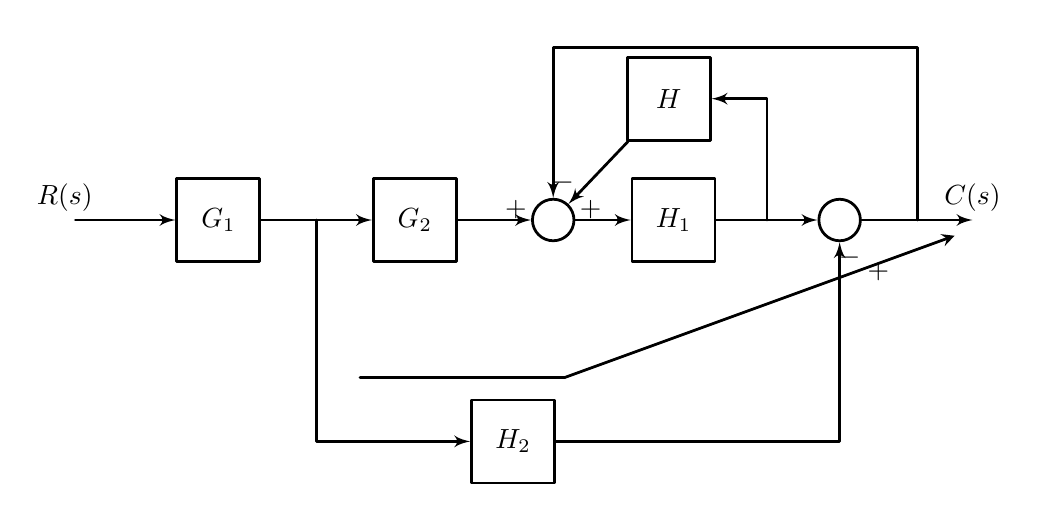
\begin{tikzpicture}
    \sbEntree{E}
    \sbBlocL[4]{a}{$G_{1}$}{E}
    \sbNomLien[0.8]{E}{$R(s)$}
    \sbBlocL[4]{b}{$G_{2}$}{a}
    
    
    \sbCompSum*[5]{T}{b}{-}{}{+}{+}
    \sbRelier{b}{T}
    \sbBlocL[2]{c}{$H_{1}$}{T}
    \sbCompSum*[6]{comp}{c}{}{-}{}{}
    \sbRelier{c}{comp}
    \sbSortie[4]{S}{comp}
    \sbRelier{comp}{S}
    \sbNomLien[0.8]{S}{$C(s)$}

    \sbDecaleNoeudy[-4]{c-comp}{node1}
    \sbBlocr{r1}{$H$}{node1}
    \sbRelieryx{c-comp}{r1}
    \sbRelier{r1}{T}
    \sbRenvoi[-7]{comp-S}{T}{}
    %\sbNomLien[2]{T}{$-$}

    \sbDecaleNoeudy[8]{b}{node2} %nodo para la segunda entrada
    \sbBloc{r2}{$H_{2}$}{node2}
    \sbRelieryx{a-b}{r2}
    \sbRelierxy{r2}{comp}
    \sbDecaleNoeudy[6]{T}{node3}
    %\sbRelieryx{a-b}{node3}
    %\sbRelier{node3}{comp}
    %\node[above of=c-comp,node distance=1cm]{$V(p)$};
    %\sbSortie[8]{r1}{T}
    %\sbRelier[$-$]{node2}{T}
    %\draw[-stealth] (node3) -- (comp)node[near end,right]{$+$};
    %lineas diagonales-->>
    \coordinate (A) at (3.75,-2);
    \coordinate (B) at (6.35,-2);
    \coordinate (C) at (11.3,-0.2);
    \draw (A) -- (B);
    \draw[-stealth] (B) -- (C)node[near end,right]{$+$};

    %\draw[-stealth] (sum.east) -- (controller.west)node[midway,above]{$e$};

    
  \end{tikzpicture}

  \begin{tikzpicture}%segundo paso ejercicio 3
     \sbEntree{E}
     \sbBlocL[4]{a}{$G_{1}$}{E}
     \sbNomLien[0.8]{E}{$R(s)$}
     \sbBlocL[4]{b}{$G_{2}$}{a}
     
     
     \sbCompSum*[5]{T1}{b}{-}{}{+}{}
     \sbRelier{b}{T1}
     \sbCompSum*[3]{T2}{T1}{+}{}{+}{}
     \sbRelier{T1}{T2}
     \sbBlocL[2]{c}{$H_{1}$}{T2}
     \sbCompSum*[6]{comp1}{c}{}{+}{+}{}
     \sbRelier{c}{comp1}
     \sbCompSum*[3]{comp2}{comp1}{}{-}{+}{}
     \sbRelier{comp1}{comp2}
     \sbSortie[4]{S}{comp2}
     \sbRelier{comp2}{S}
     \sbNomLien[0.8]{S}{$C(s)$}
     
     \sbDecaleNoeudy[-4]{c-comp1}{node1}
     \sbBlocr{r1}{$G_{3}$}{node1}
     \sbRelieryx{c-comp1}{r1} 
     \sbRelierxy{r1}{T2}
     \sbRenvoi[-7]{comp2-S}{T1}{}
     %\sbNomLien[2]{T}{$-$}
     
     \sbDecaleNoeudy[8]{T1}{node2} %nodo para la segunda entrada
     \sbBloc{r2}{$H_{2}$}{node2}
     \sbRelieryx{a-b}{r2}
     \sbRelierxy{r2}{comp2}
     \sbRenvoi[4]{a-b}{comp1}{}
     \sbDecaleNoeudy[6]{T}{node3}
     %\sbRelieryx{a-b}{node3}
     %\sbRelier{node3}{comp}
     %\node[above of=c-comp,node distance=1cm]{$V(p)$};
     %\sbSortie[8]{r1}{T}
     %\sbRelier[$-$]{node2}{T}
     %\draw[-stealth] (node3) -- (comp)node[near end,right]{$+$};
     %lineas diagonales-->>
     \coordinate (A) at (3.75,-2);
     \coordinate (B) at (6.35,-2);
     \coordinate (C) at (11.3,-0.2);
     %\draw (A) -- (B);
     %\draw[-stealth] (B) -- (C)node[near end,right]{$+$};

     %\draw[-stealth] (sum.east) -- (controller.west)node[midway,above]{$e$};

     
  \end{tikzpicture}

  \begin{tikzpicture}%tercer paso ejercicio 3
     \sbEntree{E}
     \sbBlocL[4]{a}{$G_{1}$}{E}
     \sbNomLien[0.8]{E}{$R(s)$}
     \sbBlocL[4]{b}{$G_{2}$}{a}
     
     
     \sbCompSum*[5]{T1}{b}{-}{}{+}{}
     \sbRelier{b}{T1}
     \sbBlocL[2]{c}{$\dfrac{H_{1}}{1-H_{1}G_{3}}$}{T1}
     \sbCompSum*[6]{comp1}{c}{}{+}{+}{}
     \sbRelier{c}{comp1}
     \sbCompSum*[3]{comp2}{comp1}{}{-}{+}{}
     \sbRelier{comp1}{comp2}
     \sbSortie[4]{S}{comp2}
     \sbRelier{comp2}{S}
     \sbNomLien[0.8]{S}{$C(s)$}
     
     \sbRenvoi[-4]{comp2-S}{T1}{}
     %\sbNomLien[2]{T}{$-$}
     
     \sbDecaleNoeudy[8]{T1}{node2} %nodo para la segunda entrada
     \sbBloc{r2}{$H_{2}$}{node2}
     \sbRelieryx{a-b}{r2}
     \sbRelierxy{r2}{comp2}
     \sbRenvoi[4]{a-b}{comp1}{}
     \sbDecaleNoeudy[6]{T}{node3}
     %\sbRelieryx{a-b}{node3}
     %\sbRelier{node3}{comp}
     %\node[above of=c-comp,node distance=1cm]{$V(p)$};
     %\sbSortie[8]{r1}{T}
     %\sbRelier[$-$]{node2}{T}
     %\draw[-stealth] (node3) -- (comp)node[near end,right]{$+$};
     %lineas diagonales-->>
     \coordinate (A) at (3.75,-2);
     \coordinate (B) at (6.35,-2);
     \coordinate (C) at (11.3,-0.2);
     %\draw (A) -- (B);
     %\draw[-stealth] (B) -- (C)node[near end,right]{$+$};

     %\draw[-stealth] (sum.east) -- (controller.west)node[midway,above]{$e$};

     
  \end{tikzpicture}

  \begin{tikzpicture}%tercer paso ejercicio 3
     \sbEntree{E}
     \sbBlocL[4]{a}{$G_{1}$}{E}
     \sbNomLien[0.8]{E}{$R(s)$}
     \sbBlocL[4]{b}{$G_{2}$}{a}
     \sbBlocL[2]{c}{$\dfrac{H_{1}}{1-H_{1}G_{3}}$}{b}
     
     \sbCompSum*[5]{T1}{c}{-}{}{+}{}
     \sbRelier{c}{T1}
     \sbCompSum*[4]{comp1}{T1}{}{+}{+}{}
     \sbRelier{T1}{comp1}
     \sbCompSum*[4]{comp2}{comp1}{}{-}{+}{}
     \sbRelier{comp1}{comp2}
     \sbSortie[4]{S}{comp2}
     \sbRelier{comp2}{S}
     \sbNomLien[0.8]{S}{$C(s)$}
     

     \sbDecaleNoeudy[-5]{comp2-S}{node1}
     \sbBlocr[2]{d}{$\dfrac{H_{1}}{1-H_{1}G_{3}}$}{node1}
     \sbRelierxy{d}{T1}
     \sbRelieryx{comp2-S}{d}
     %\sbNomLien[2]{T}{$-$}
     
     \sbDecaleNoeudy[8]{T1}{node2} %nodo para la segunda entrada
     \sbBloc{r2}{$H_{2}$}{node2}
     \sbRelieryx{a-b}{r2}
     \sbRelierxy{r2}{comp2}
     \sbRenvoi[4]{a-b}{comp1}{}
     \sbDecaleNoeudy[6]{T}{node3}
     %\sbRelieryx{a-b}{node3}
     %\sbRelier{node3}{comp}
     %\node[above of=c-comp,node distance=1cm]{$V(p)$};
     %\sbSortie[8]{r1}{T}
     %\sbRelier[$-$]{node2}{T}
     %\draw[-stealth] (node3) -- (comp)node[near end,right]{$+$};
     %lineas diagonales-->>
     \coordinate (A) at (3.75,-2);
     \coordinate (B) at (6.35,-2);
     \coordinate (C) at (11.3,-0.2);
     %\draw (A) -- (B);
     %\draw[-stealth] (B) -- (C)node[near end,right]{$+$};

     %\draw[-stealth] (sum.east) -- (controller.west)node[midway,above]{$e$};

     
  \end{tikzpicture}

  \begin{tikzpicture}%cuarto paso ejercicio 3
     \sbEntree{E}
     \sbBlocL[4]{a}{$G_{1}$}{E}
     \sbNomLien[0.8]{E}{$R(s)$}
     \sbBlocL[4]{b}{$G_{2}$}{a}
     \sbBlocL[2]{c}{$\dfrac{H_{1}}{1-H_{1}G_{3}}$}{b}
     
     \sbCompSum*[6]{comp1}{c}{}{+}{+}{}
     \sbRelier{c}{comp1}
     \sbCompSum*[4]{comp2}{comp1}{}{-}{+}{}
     \sbRelier{comp1}{comp2}
     \sbCompSum*[4]{T1}{comp2}{-}{}{+}{}
     \sbRelier{comp2}{T1}
     \sbSortie[8]{S}{T1}
     \sbRelier{T1}{S}
     \sbNomLien[0.8]{S}{$C(s)$}
     

     \sbDecaleNoeudy[-5]{S}{node1}
     \sbBlocr[2]{d}{$\dfrac{H_{1}}{1-H_{1}G_{3}}$}{node1}
     %\sbRelieryx{T1-S}{d}
     \sbRelierxy{d}{T1}
     %\sbNomLien[2]{T}{$-$}
     
     \sbDecaleNoeudy[8]{c}{node2} %nodo para la segunda entrada
     \sbBloc{r2}{$H_{2}$}{node2}
     \sbRelieryx{a-b}{r2}
     \sbRelierxy{r2}{comp2}
     \sbRenvoi[4]{a-b}{comp1}{}
     \sbDecaleNoeudy[6]{T}{node3}
     %\sbRelieryx{a-b}{node3}
     %\sbRelier{node3}{comp}
     %\node[above of=c-comp,node distance=1cm]{$V(p)$};
     %\sbSortie[8]{r1}{T}
     %\sbRelier[$-$]{node2}{T}
     %\draw[-stealth] (node3) -- (comp)node[near end,right]{$+$};
     %lineas diagonales-->>

     \coordinate (A) at (16.65,0);
     \coordinate (B) at (16.34,2.1);
     \draw (A) |- (B);
     %\draw[-stealth] (B) -- (C)node[near end,right]{$+$};

     %\draw[-stealth] (sum.east) -- (controller.west)node[midway,above]{$e$};

     
  \end{tikzpicture}

  \vspace{1cm}

  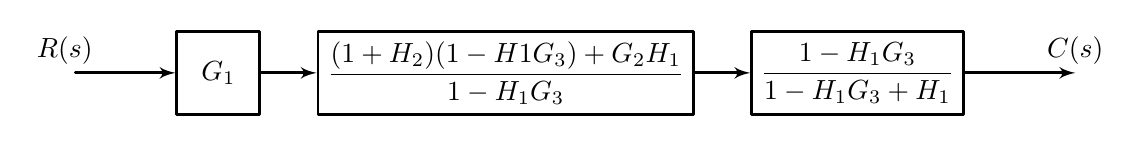
\begin{tikzpicture}quinto paso ejercicio 3
     \sbEntree{E}
     \sbBlocL[4]{a}{$G_{1}$}{E}
     \sbNomLien[0.8]{E}{$R(s)$}
     \sbBlocL[2]{b}{$\dfrac{(1+H_{2})(1-H{1}G_{3})+G_{2}H_{1}}{1-H_{1}G_{3}}$}{a}
     \sbBlocL[2]{c}{$\dfrac{1-H_{1}G_{3}}{1-H_{1}G_{3}+H_{1}}$}{b}
     \sbSortie[4]{S}{c}
     \sbRelier{c}{S}
     \sbNomLien[0.8]{S}{$C(s)$}

     %\coordinate (A) at (16.65,0);
     %\coordinate (B) at (16.34,2.1);
     %\draw (A) |- (B);
     %\draw[-stealth] (B) -- (C)node[near end,right]{$+$};
     %\draw[-stealth] (sum.east) -- (controller.west)node[midway,above]{$e$};
     
  \end{tikzpicture}

  \vspace{1cm}

  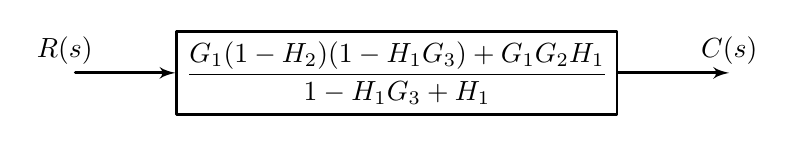
\begin{tikzpicture}quinto paso ejercicio 3
     \sbEntree{E}
     \sbBlocL[4]{a}{$\dfrac{G_{1}(1-H_{2})(1-H_{1}G_{3})+G_{1}G_{2}H_{1}}{1-H_{1}G_{3}+H_{1}}$}{E}
     \sbNomLien[0.8]{E}{$R(s)$}
     \sbSortie[4]{S}{a}
     \sbRelier{a}{S}
     \sbNomLien[0.8]{S}{$C(s)$}

     %\coordinate (A) at (16.65,0);
     %\coordinate (B) at (16.34,2.1);
     %\draw (A) |- (B);
     %\draw[-stealth] (B) -- (C)node[near end,right]{$+$};
     %\draw[-stealth] (sum.east) -- (controller.west)node[midway,above]{$e$};
     
  \end{tikzpicture}


\newpage

\section*{Ejercicio \# 4}

Hallar: \(\displaystyle C(s)=?\)

  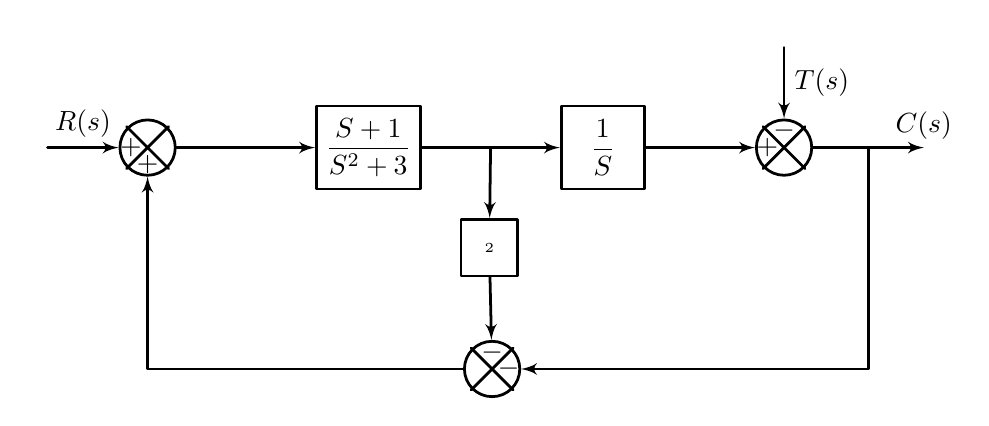
\begin{tikzpicture}
     \sbEntree{E}
     \sbSumb{a}{E}
     \sbRelier[$R(s)$]{E}{a}
     \sbBlocL[5]{b}{$\dfrac{S+1}{S^{2}+3}$}{a}
     \sbBlocL[5]{c}{$\dfrac{1}{S}$}{b}
     
     \sbComph[5]{T}{c}
     \sbRelier{c}{T}
     \sbSortie[4]{S}{T}
     \sbRelier{T}{S}
     \sbNomLien[0.8]{S}{$C(s)$}
    
     \sbDecaleNoeudy[8]{c}{u}
     \sbCompSum[-4]{C1}{u}{-}{}{}{-}
     \sbRelieryx{T-S}{C1}
     \sbRelierxy{C1}{a}

     %REVISAR CODIGO
     \sbDecaleNoeudy[0]{b-c}{y2}
     \sbDecaleNoeudy[4]{b-c}{y3}
     \sbDecaleNoeudy[0]{b-c}{y4}
     \begin{tiny}
     \sbBlocr[-1.5]{y2}{$2$}{y3}
     \end{tiny}
     \sbRelier{y2}{C1}
     \sbRelier{y4}{y2}
     
    
     \sbDecaleNoeudy[-4]{T}{y} %nodo para la segunda entrada
     \sbRelier[$T(s)$]{y}{T}
                
  \end{tikzpicture}

primero ordenamos un poco.

  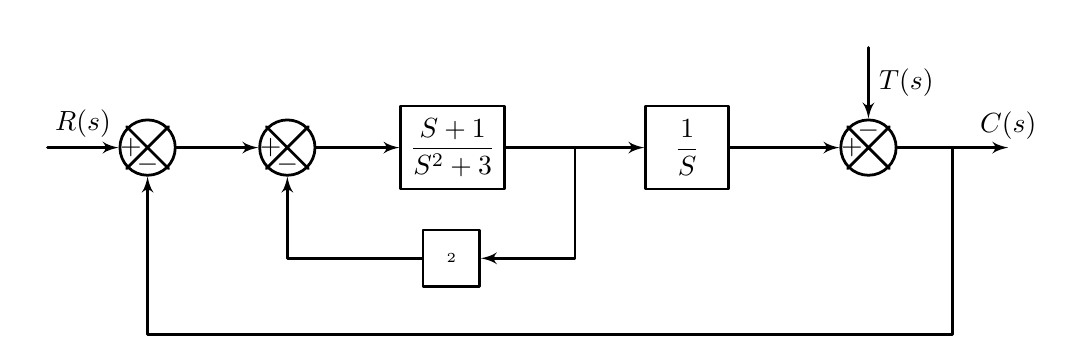
\begin{tikzpicture}
     \sbEntree{E}
     \sbCompSum{C1}{E}{}{-}{+}{}
     \sbRelier[$R(s)$]{E}{C1}
     \sbCompSum[4]{C2}{C1}{}{-}{+}{}
     \sbRelier{C1}{C2}
     \sbBlocL[3]{a}{$\dfrac{S+1}{S^{2}+3}$}{C2}
     \sbBlocL[5]{b}{$\dfrac{1}{S}$}{a}
     
     \sbComph[5]{T}{b}
     \sbRelier{b}{T}
     \sbSortie[4]{S}{T}
     \sbRelier{T}{S}
     \sbNomLien[0.8]{S}{$C(s)$}
    

     %REVISAR CODIGO
     %\sbDecaleNoeudy[0]{C2}{y2}
     \sbDecaleNoeudy[4]{a}{y3}
     %\sbDecaleNoeudy[0]{b-c}{y4}
     \begin{tiny}
     \sbBlocr[-1.5]{y2}{$2$}{y3}
     \end{tiny}
     \sbRelieryx{a-b}{y2}
     \sbRelierxy{y2}{C2}
     
     \sbRenvoi[6]{T-S}{C1}{}
    
     \sbDecaleNoeudy[-4]{T}{y} %nodo para la segunda entrada
     \sbRelier[$T(s)$]{y}{T}
                
  \end{tikzpicture}


  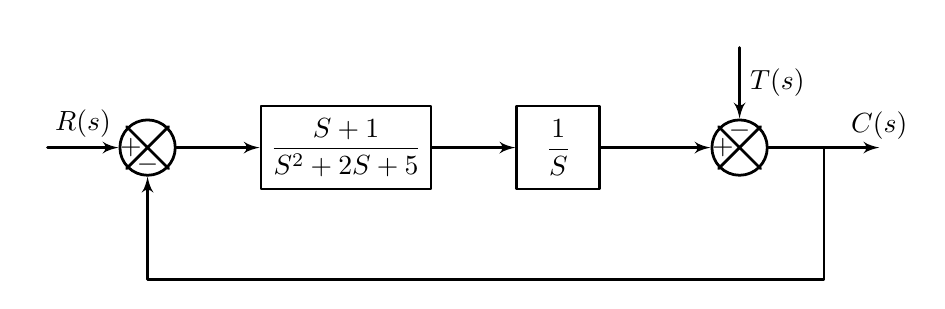
\begin{tikzpicture}
     \sbEntree{E}
     \sbCompSum{C1}{E}{}{-}{+}{}
     \sbRelier[$R(s)$]{E}{C1}
     \sbBlocL[3]{a}{$\dfrac{S+1}{S^{2}+2S+5}$}{C1}
     \sbBlocL[3]{b}{$\dfrac{1}{S}$}{a}
     
     \sbComph[5]{T}{b}
     \sbRelier{b}{T}
     \sbSortie[4]{S}{T}
     \sbRelier{T}{S}
     \sbNomLien[0.8]{S}{$C(s)$}
    
     
     \sbRenvoi[4]{T-S}{C1}{}
    
     \sbDecaleNoeudy[-4]{T}{y} %nodo para la segunda entrada
     \sbRelier[$T(s)$]{y}{T}
                
  \end{tikzpicture}

  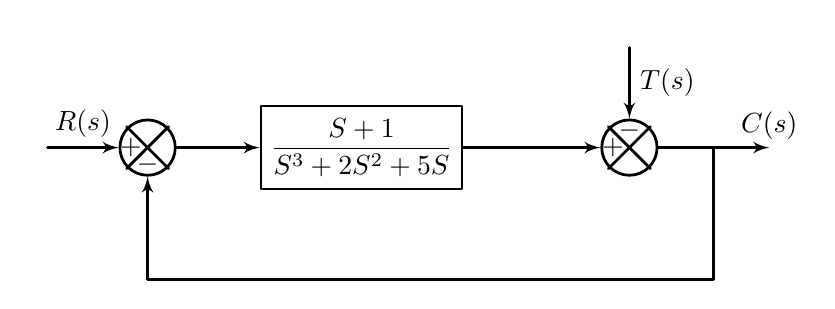
\begin{tikzpicture}
     \sbEntree{E}
     \sbCompSum{C1}{E}{}{-}{+}{}
     \sbRelier[$R(s)$]{E}{C1}
     \sbBlocL[3]{a}{$\dfrac{S+1}{S^{3}+2S^{2}+5S}$}{C1}
     
     \sbComph[6]{T}{a}
     \sbRelier{a}{T}
     \sbSortie[4]{S}{T}
     \sbRelier{T}{S}
     \sbNomLien[0.8]{S}{$C(s)$}
     
     \sbRenvoi[4]{T-S}{C1}{}
    
     \sbDecaleNoeudy[-4]{T}{y} %nodo para la segunda entrada
     \sbRelier[$T(s)$]{y}{T}
                
  \end{tikzpicture}

\vspace{1cm}

Luego por superposici'on hacemos \(\displaystyle T(s)=0\)

  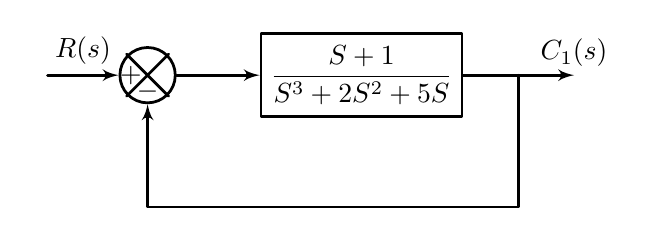
\begin{tikzpicture}
     \sbEntree{E}
     \sbCompSum{C1}{E}{}{-}{+}{}
     \sbRelier[$R(s)$]{E}{C1}
     \sbBlocL[3]{a}{$\dfrac{S+1}{S^{3}+2S^{2}+5S}$}{C1}
     
     %\sbComph[6]{T}{a}
     %\sbRelier{a}{T}
     \sbSortie[4]{S}{a}
     \sbRelier{a}{S}
     \sbNomLien[0.8]{S}{$C_{1}(s)$}
     
     \sbRenvoi[4]{a-S}{C1}{}
    
     %\sbDecaleNoeudy[-4]{T}{y} %nodo para la segunda entrada
     %\sbRelier[$T(s)$]{y}{T}
                
  \end{tikzpicture}

  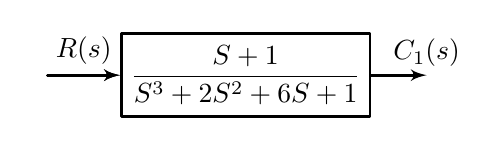
\begin{tikzpicture}
     \sbEntree{E}
     \sbBlocL[3]{a}{$\dfrac{S+1}{S^{3}+2S^{2}+6S+1}$}{E}
     \sbRelier[$R(s)$]{E}{a}
     
     %\sbComph[6]{T}{a}
     %\sbRelier{a}{T}
     \sbSortie[2]{S}{a}
     \sbRelier{a}{S}
     \sbNomLien[0.8]{S}{$C_{1}(s)$}
     
    
     %\sbDecaleNoeudy[-4]{T}{y} %nodo para la segunda entrada
     %\sbRelier[$T(s)$]{y}{T}
                
  \end{tikzpicture}

  \vspace{1cm}

  Luego por superposici'on hacemos \(\displaystyle R(s)=0\)

  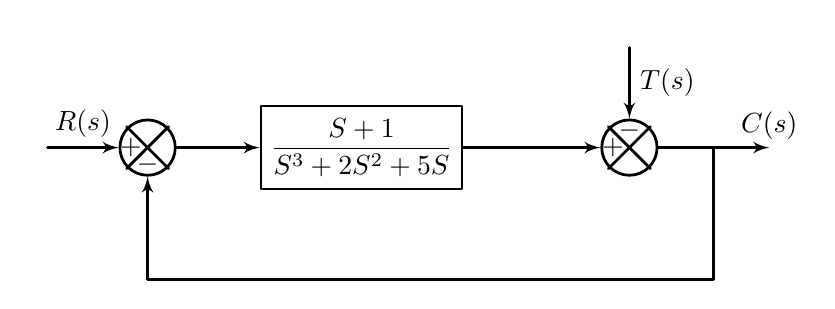
\begin{tikzpicture}
     \sbEntree{E}
     \sbCompSum{C1}{E}{}{-}{+}{}
     \sbRelier[$R(s)$]{E}{C1}
     \sbBlocL[3]{a}{$\dfrac{S+1}{S^{3}+2S^{2}+5S}$}{C1}
     
     \sbComph[6]{T}{a}
     \sbRelier{a}{T}
     \sbSortie[4]{S}{T}
     \sbRelier{T}{S}
     \sbNomLien[0.8]{S}{$C(s)$}
     
     \sbRenvoi[4]{T-S}{C1}{}
    
     \sbDecaleNoeudy[-4]{T}{y} %nodo para la segunda entrada
     \sbRelier[$T(s)$]{y}{T}
                
  \end{tikzpicture}

   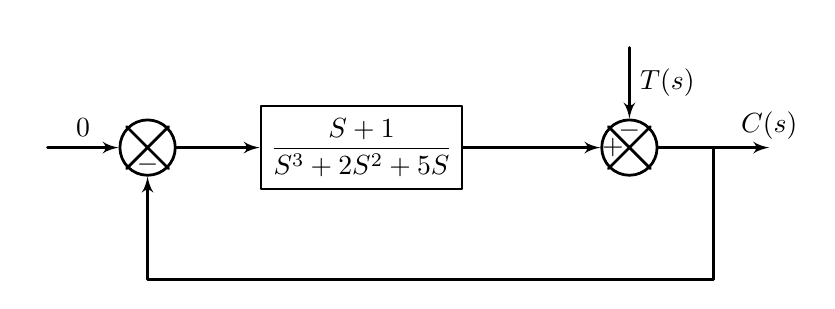
\begin{tikzpicture}
     \sbEntree{E}
     \sbCompSum{C1}{E}{}{-}{}{}
     \sbRelier[$0$]{E}{C1}
     \sbBlocL[3]{a}{$\dfrac{S+1}{S^{3}+2S^{2}+5S}$}{C1}
     
     \sbComph[6]{T}{a}
     \sbRelier{a}{T}
     \sbSortie[4]{S}{T}
     \sbRelier{T}{S}
     \sbNomLien[0.8]{S}{$C(s)$}
     
     \sbRenvoi[4]{T-S}{C1}{}
    
     \sbDecaleNoeudy[-4]{T}{y} %nodo para la segunda entrada
     \sbRelier[$T(s)$]{y}{T}
                
  \end{tikzpicture}
   
  \vspace{1cm}

 \begin{tikzpicture}
   \sbEntree{E}
   \sbCompSum{C1}{E}{}{+}{-}{}
   \sbRelier[$T(s)$]{E}{C1}
   %\sbBlocL[3]{a}{$\dfrac{S+1}{S^{3}+2S^{2}+5S}$}{C1}
   
   %\sbComph[6]{T}{a}
   %\sbRelier{a}{T}
   \sbSortie[16]{S}{C1}
   \sbRelier{C1}{S}
   \sbNomLien[0.8]{S}{$C_{2}(s)$}
   
   %\sbRenvoi[4]{T-S}{C1}{$-1$}
  
   \sbDecaleNoeudy[4]{a-S}{y} %nodo para la segunda entrada
   \begin{tiny}
   \sbBlocr[-6.5]{a}{$-1$}{y}
   \end{tiny}
   \sbBlocr[-1]{a}{$\dfrac{S+1}{S^{3}+2S^{2}+5S}$}{y}
   %\sbRelieryx[$R(s)$]{a}{y}
   %\sbRelier[$T(s)$]{y}{T}

  \coordinate (A) at (8,0);
  \coordinate (B) at (7.05,-1.5);
  \coordinate (C) at (6.22,-1.5);
  \coordinate (D) at (5.75,-1.5);
  \coordinate (E) at (1.67,-0.4);
  \coordinate (F) at (2.8,-1.5);
  \draw (A) |- (B);
  \draw (C) -- (D);
   \draw[-stealth] (F) -| (E);
     %\draw[-stealth] (B) -- (C)node[near end,right]{$+$};
     %\draw[-stealth] (sum.east) -- (controller.west)node[midway,above]{$e$};
              
\end{tikzpicture}

\vspace{1cm}

 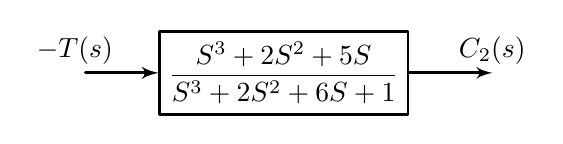
\begin{tikzpicture}
   \sbEntree{E}
   \sbBlocL[3]{a}{$\dfrac{S^{3}+2S^{2}+5S}{S^{3}+2S^{2}+6S+1}$}{E}
   \sbRelier[$$]{E}{a}
   \sbNomLien[0.8]{E}{$-T(s)$}
   
   \sbSortie[3]{S}{a}
   \sbRelier{a}{S}
   \sbNomLien[0.8]{S}{$C_{2}(s)$}
   
\end{tikzpicture}

\vspace{1cm}
Superposici'on de las salidas \(\displaystyle C(s)=C_{1}(s)+C_{2}(s)\)

\begin{eqnarray*}
  C(s) &=& R(s)\dfrac{S+1}{S^{3}+2S^{2}+6S+1}-T(s)\dfrac{S^{3}+2S^{2}+5S}{S^{3}+2S^{2}+6S+1}
\end{eqnarray*}

\newpage

\section*{Ejercicio \# 5}
%Ejercicio # 5
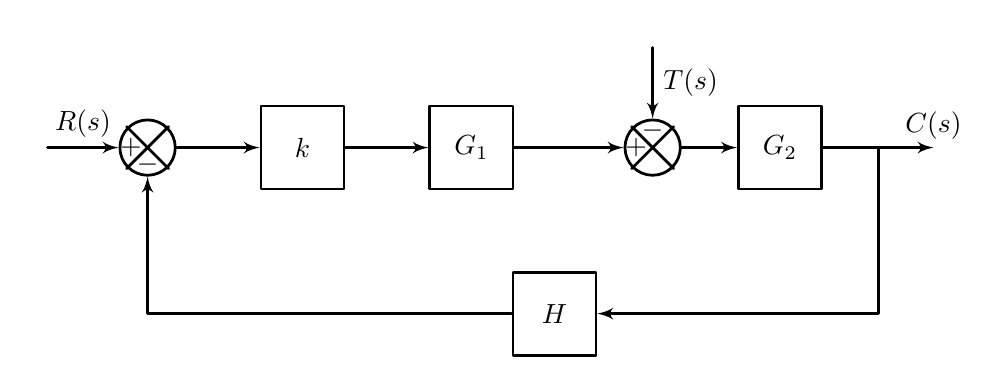
\begin{tikzpicture}
        \sbEntree{E}
        \sbComp{a}{E}
        \sbRelier[$R(s)$]{E}{a}
        \sbBlocL[3]{b}{$k$}{a}
        \sbBlocL[3]{c}{$G_{1}$}{b}
        
        \sbComph[5]{T}{c}
        \sbRelier{c}{T}
        \sbBlocL[2]{d}{$G_{2}$}{T}
        \sbSortie[4]{S}{d}
        \sbRelier{d}{S}
        \sbNomLien[0.8]{S}{$C(s)$}

        \sbDecaleNoeudy[6]{T}{u}
        \sbBlocr{r1}{$H$}{u}
        \sbRelieryx{d-S}{r1}
        \sbRelierxy{r1}{a}

        \sbDecaleNoeudy[-4]{T}{y} %nodo para la segunda entrada
        \sbRelier[$T(s)$]{y}{T}
        
\end{tikzpicture}

Por superposici'on hacemos \(\displaystyle T(s)=0\).

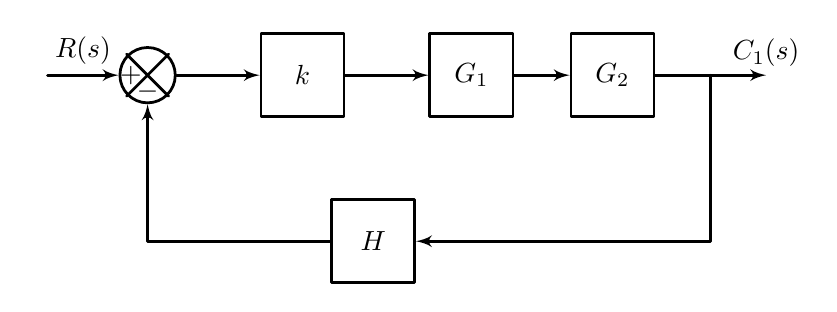
\begin{tikzpicture}
        \sbEntree{E}
        \sbComp{a}{E}
        \sbRelier[$R(s)$]{E}{a}
        \sbBlocL[3]{b}{$k$}{a}
        \sbBlocL[3]{c}{$G_{1}$}{b}
        
        %\sbComph[5]{T}{c}
        %\sbRelier{c}{T}
        \sbBlocL[2]{d}{$G_{2}$}{c}
        \sbSortie[4]{S}{d}
        \sbRelier{d}{S}
        \sbNomLien[0.8]{S}{$C_{1}(s)$}

        \sbDecaleNoeudy[6]{c}{u}
        \sbBlocr{r1}{$H$}{u}
        \sbRelieryx{d-S}{r1}
        \sbRelierxy{r1}{a}

        %\sbDecaleNoeudy[-4]{T}{y} %nodo para la segunda entrada
        %\sbRelier[$T(s)$]{y}{T}
        
\end{tikzpicture}

\vspace{1cm}

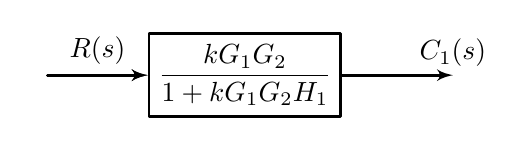
\begin{tikzpicture}
        \sbEntree{E}
        \sbBlocL[4]{a}{$\dfrac{kG_{1}G_{2}}{1+kG_{1}G_{2}H_{1}}$}{E}
        \sbRelier[$R(s)$]{E}{a}
        
        \sbSortie[4]{S}{a}
        \sbRelier{a}{S}
        \sbNomLien[0.8]{S}{$C_{1}(s)$}
        
\end{tikzpicture}

\vspace{1cm}

Por superposici'on hacemos \(\displaystyle R(s)=0\).

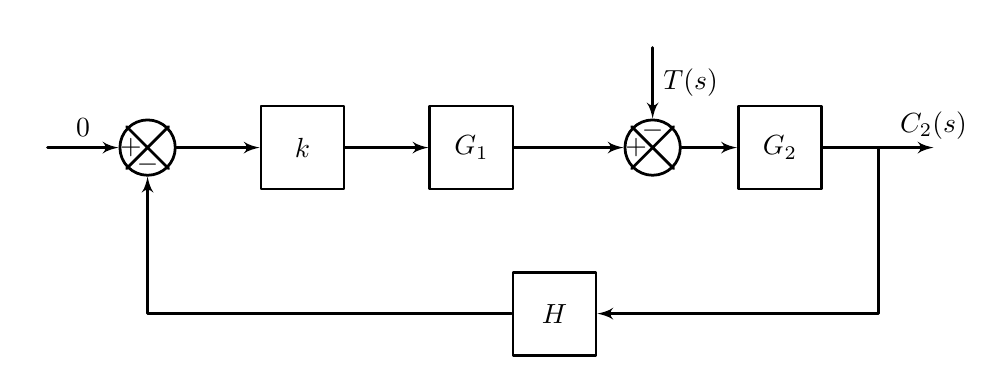
\begin{tikzpicture}
        \sbEntree{E}
        \sbComp{a}{E}
        \sbRelier[$0$]{E}{a}
        \sbBlocL[3]{b}{$k$}{a}
        \sbBlocL[3]{c}{$G_{1}$}{b}
        
        \sbComph[5]{T}{c}
        \sbRelier{c}{T}
        \sbBlocL[2]{d}{$G_{2}$}{T}
        \sbSortie[4]{S}{d}
        \sbRelier{d}{S}
        \sbNomLien[0.8]{S}{$C_{2}(s)$}

        \sbDecaleNoeudy[6]{T}{u}
        \sbBlocr{r1}{$H$}{u}
        \sbRelieryx{d-S}{r1}
        \sbRelierxy{r1}{a}

        \sbDecaleNoeudy[-4]{T}{y} %nodo para la segunda entrada
        \sbRelier[$T(s)$]{y}{T}
        
\end{tikzpicture}

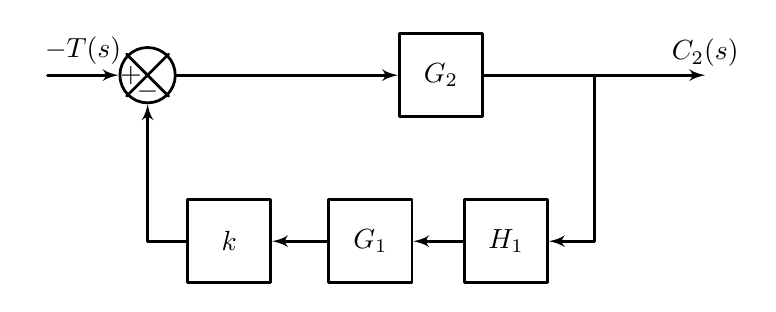
\begin{tikzpicture}
        \sbEntree{E}
        \sbComp{a}{E}
        \sbRelier[$-T(s)$]{E}{a}
        \sbBlocL[8]{b}{$G_{2}$}{a}
        
        \sbSortie[8]{S}{b}
        \sbRelier{b}{S}
        \sbNomLien[0.8]{S}{$C_{2}(s)$}

        \sbDecaleNoeudy[6]{b}{u}
        \sbBlocr[1]{r1}{$G_{1}$}{u}
        \sbBlocr[2]{r2}{$k$}{r1}
        \sbBlocr[-8]{r3}{$H_{1}$}{r1}
        \sbRelieryx{b-S}{r3}
        \sbRelier{r3}{r1}
        \sbRelier{r1}{r2}
        \sbRelierxy{r2}{a}

        %\sbDecaleNoeudy[-4]{T}{y} %nodo para la segunda entrada
        %\sbRelier[$T(s)$]{y}{T}
        
\end{tikzpicture}

\vspace{1cm}

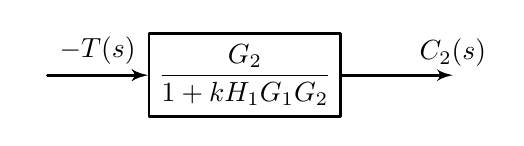
\begin{tikzpicture}
        \sbEntree{E}
        \sbBlocL[4]{a}{$\dfrac{G_{2}}{1+kH_{1}G_{1}G_{2}}$}{E}
        \sbRelier[$-T(s)$]{E}{a}
        
        \sbSortie[4]{S}{a}
        \sbRelier{a}{S}
        \sbNomLien[0.8]{S}{$C_{2}(s)$}
        
\end{tikzpicture}

\vspace{1cm}
Superposici'on de las salidas \(\displaystyle C(s)=C_{1}(s)+C_{2}(s)\)

\begin{eqnarray*}
  C(s) &=& R(s)\dfrac{kG_{1}G_{2}}{1+kH_{1}G_{1}G_{2}}-T(s)\dfrac{G_{2}}{1+kH_{1}G_{1}G_{2}}
\end{eqnarray*}

\newpage

\section*{Ejercicio \# 6}

\setcounter{equation}{0}

Hallar: \(\displaystyle FT=\frac{H_{2}(s)}{Q_{in}(s)} \hspace{5mm} ; \hspace{5mm} FT=\frac{Q_{2}(s)}{Q_{in}(s)}\)

\tikzset{
    pics/.cd,
    reservoir/.style={
        code={
            \fill[rounded corners,blue!50]  (-1,#1-1)--(-1,-1)--(1,-1)--(1,#1-1);
            \draw[rounded corners](-1.1,1)--(-1,.9)--(-1,-1)--(1,-1)--(1,.9)--(1.1,1);
        }
    },
    right valve/.style={
        code={
            \fill[blue!50](-.1, .1)--(.2, .1)arc(90:0:.2)        --(-.1,-.1);
            \draw         (-.1, .1)--(.2, .1)arc(90:0:.2)(.2,-.1)--(-.1,-.1);
            \fill(.1, .1)+(-.05,0)--+(.05,0)--+(0,-.07)
                 (.1,-.1)+(-.05,0)--+(.05,0)--+(0, .07);
            \draw[blue!50,line width=.2cm,domain=0:#1,samples=#1*10,shift={(.3,-.3)}]
                 (0,.2)--(0,.1)--plot({rand/30},-\x);
        }
    },
    left valve/.style={
        /tikz/xscale=-1,right valve=#1
    },
    pipe/.style={
        code={
            \fill[blue!50](-#1-.1,.1)rectangle(#1+.1,-.1);
            \draw         (-#1-.1,.1)--(#1+.1,.1)(-#1-.1,-.1)--(#1+.1,-.1);
            \fill(0, .1)+(-.05,0)--+(.05,0)--+(0,-.07)
                 (0,-.1)+(-.05,0)--+(.05,0)--+(0, .07);
        }
    }
}

\tikzset{
    pics/labeled right valve/.style n args={3}{
        code={
            \fill[blue!50](-.1, .1)--(.2, .1)arc(90:0:.2)        --(-.1,-.1);
            \draw         (-.1, .1)--(.2, .1)arc(90:0:.2)(.2,-.1)--(-.1,-.1);
            \fill(.1, .1)+(-.05,0)--+(.05,0)--+(0,-.07)
                 (.1,-.1)+(-.05,0)--+(.05,0)--+(0, .07)
                 (.2, .1)node[above]{$#2$};
            \draw[blue!50,line width=.2cm,domain=0:#1,samples=#1*10,shift={(.3,-.3)}]
                 (0,.2)--(0,.1)--plot({rand/30},-\x)node[above right,black]{$#3$};
        }
    },
}

\tikzset{
    pics/labeled reservoir/.style 2 args={
        code={
            \fill[rounded corners,blue!50]  (-1,#1-1)--(-1,-1)--(1,-1)--(1,#1-1);
            \draw[rounded corners](-1.1,1)--(-1,.9)--(-1,-1)--(1,-1)--(1,.9)--(1.1,1);
            \draw[->](0,-.9)--(0,#1-1)node[below right]{$#2$};
        }
    },
}


%\tikz{
%    \path                                               (4,6  )pic{reservoir=1.5}
%         (-3,6.5)pic{right valve=2}                     (3,5.5)pic{left valve=2.2}
%         (-2,3  )pic{reservoir=1.8}                     (2,3  )pic{reservoir=.7}
%                                    (0,2.5)pic{pipe={1}}
%         (-3,2.5)pic{left valve=2.7}                    (3,2.5)pic{right valve=1.6}
%         (-4,0  )pic{reservoir=.2}                      (4,0  )pic{reservoir=1.1}
%    ;
%}
\vspace{1cm}

%\tikz{
%    \path
%        (-3.2,5)pic{pipe=0.2} (-3,5)pic{labeled right valve={0.8}{}{q_{in}(t)}}
%        (-2,3  )pic{labeled reservoir={1.5}{h_{1}(t)}} (-0.7,2.2)pic{pipe=0.2} (-0.3,2.2)pic{labeled right valve={0.8}{R_{1}}{q_{1}(t)}}
%        (0.8,0.5   )pic{labeled reservoir={1}{h_{2}(t)}} (2.1,-0.2)pic{pipe=0.2} (2.2,-0.2)pic{labeled right valve={0.5}{R_{2}}{q_{2}(t)}}  
%}

%Tanque de agua con altura
%\tikz{
%    \path pic{labeled reservoir={1.3}{h_3}};
%}

%valvula con Q y R

%\tikz{
%    \path pic{labeled right valve={1.3}{R_4}{Q_4}};
%}
\begin{tikzpicture} 
  \path
        (-3.2,5)pic{pipe=0.2} (-3,5)pic{labeled right valve={0.8}{}{q_{in}(t)}}
        (-2,3  )pic{labeled reservoir={1.5}{h_{1}(t)}} (-0.7,2.2)pic{pipe=0.2} (-0.3,2.2)pic{labeled right valve={0.8}{R_{1}}{q_{1}(t)}}
        (0.8,0.5   )pic{labeled reservoir={1.2}{h_{2}(t)}} (2.1,-0.2)pic{pipe=0.2} (2.2,-0.2)pic{labeled right valve={0.5}{R_{2}}{q_{2}(t)}}  

    ;

  \coordinate (A) at (-3,1.8);
  \coordinate (B) at (-1,1.8);
  \coordinate (C) at (-0.2,-0.7);
  \coordinate (D) at ( 1.8,-0.7);

  \draw[<->] (A) -- (B)node[midway,below]{$A_{1}$};
  \draw[<->] (C) -- (D)node[midway,below]{$A_{2}$};
\end{tikzpicture}

Soluci\'on:

\begin{enumerate}
  \item Primero analisamos el primer tanque de agua.\\

    \begin{tikzpicture} 
      \path
            (-3.2,5)pic{pipe=0.2} (-3,5)pic{labeled right valve={0.8}{}{q_{in}(t)}}
            (-2,3  )pic{labeled reservoir={1.5}{h_{1}(t)}} (-0.7,2.2)pic{pipe=0.2} (-0.3,2.2)pic{labeled right valve={0.8}{R_{1}}{q_{1}(t)}}
            (0.8,0.5   )  

        ;

      \coordinate (A) at (-3,1.8);
      \coordinate (B) at (-1,1.8);
      \coordinate (C) at (-0.2,-0.7);
      \coordinate (D) at ( 1.8,-0.7);

      \draw[<->] (A) -- (B)node[midway,below]{$A_{1}$};
      
    \end{tikzpicture}

    En el tanque 1 tenemos: 

    \(\displaystyle V_{1}(t)=A_{1}h_{1}(t)\)

    \( \displaystyle \frac{dV_{1}(t)}{dt}=A_{1}\frac{dh_{1}(t)}{dt} \)

    \( \displaystyle q_{in}(t)-q_{1}(t) = A_{1}\frac{dh_{1}(t)}{dt} \)

    Luego tenemos que el caudal de salida del primer tanque $q_{1}(t)$ es inverzamente
    proporcional a la resitencia de la valvula $R_{1}$ y directamente proporcional a $h_{1}(t)$.

    \( \displaystyle q_{1}(t)=\frac{1}{R_{1}}h_{1}(t)\)

    Entonces tenemos el siguiente sistema de ecuaciones:

    \begin{eqnarray}
      q_{in}(t)-q_{1}(t) &=& A_{1}\frac{dh_{1}(t)}{dt} \\
      q_{1}(t) &=& \frac{1}{R_{1}}h_{1}(t)
    \end{eqnarray}

    Luego aplicamos la transformada de Laplace:
 
    \begin{eqnarray*}
      \mathscr{L}\{q_{in}(t)-q_{1}(t)\} &=& \mathscr{L} \left\{ A_{1}\frac{dh_{1}(t)}{dt} \right\} \\[2mm]
      \mathscr{L}\{q_{1}(t)\} &=&\mathscr{L} \left \{ \frac{1}{R_{1}}h_{1}(t) \right\}
    \end{eqnarray*}

\setcounter{equation}{0}
    \begin{eqnarray}
      Q_{in}(s) - Q_{1}(s) &=& A_{1}SH_{1}(s) \\[2mm]
      Q_{1}(s) &=& \frac{1}{R_{1}}H_{1}(s)
    \end{eqnarray}
  \item Ahora nalizamos el segundo tanque.\\

    \begin{tikzpicture} 
      \path
            (-0.7,2.2)pic{pipe=0.2} (-0.3,2.2)pic{labeled right valve={0.8}{R_{1}}{q_{1}(t)}}
            (0.8,0.5   )pic{labeled reservoir={1.2}{h_{2}(t)}} (2.1,-0.2)pic{pipe=0.2} (2.2,-0.2)pic{labeled right valve={0.5}{R_{2}}{q_{2}(t)}}  

        ;

      \coordinate (A) at (-3,1.8);
      \coordinate (B) at (-1,1.8);
      \coordinate (C) at (-0.2,-0.7);
      \coordinate (D) at ( 1.8,-0.7);

      \draw[<->] (C) -- (D)node[midway,below]{$A_{2}$};
    \end{tikzpicture}

    En el tanque 2 tenemos: 

    \(\displaystyle V_{2}(t)=A_{2}h_{2}(t)\)

    \( \displaystyle \frac{dV_{2}(t)}{dt}=A_{2}\frac{dh_{2}(t)}{dt} \)

    \( \displaystyle q_{1}(t)-q_{2}(t) = A_{2}\frac{dh_{2}(t)}{dt} \)

    Luego tenemos que el caudal de salida del segundo tanque $q_{2}(t)$ es inverzamente
    proporcional a la resitencia de la valvula $R_{2}$ y directamente proporcional a $h_{2}(t)$.

    \( \displaystyle q_{2}(t)=\frac{1}{R_{2}}h_{2}(t)\)

    Entonces tenemos el siguiente sistema de ecuaciones:

    \begin{eqnarray*}
      q_{1}(t) - q_{2}(t) &=& A_{2}\frac{dh_{2}(t)}{dt} \\
      q_{2}(t) &=& \frac{1}{R_{2}}h_{2}(t)
    \end{eqnarray*}

    Luego aplicamos la transformada de Laplace:
 
    \begin{eqnarray*}
      \mathscr{L}\{q_{1}(t) - q_{2}(t)\} &=& \mathscr{L} \left\{ A_{2}\frac{dh_{2}(t)}{dt} \right\} \\[2mm]
      \mathscr{L}\{q_{2}(t)\} &=&\mathscr{L} \left \{ \frac{1}{R_{2}}h_{2}(t) \right\}
    \end{eqnarray*}

    \begin{eqnarray}
      Q_{1}(s) - Q_{2}(s) &=& A_{2}SH_{2}(s) \\[2mm]
      Q_{2}(s) &=& \frac{1}{R_{2}}H_{2}(s)
    \end{eqnarray}

  \item Luego hacemos (2) en (1) y (4) en (3) \\

    De (1) \hspace{5mm} \(\displaystyle Q_{in}(s)=A_{1}SH_{1}(s)+Q_{1}(s)\)

    remplazamos (2) en (1)

   \(\displaystyle Q_{in}(s)=A_{1}SQ_{1}(s)R_{1}+Q_{1}(s)\)\\

   \(\displaystyle Q_{in}(s)=Q_{1}(s)[A_{1}SR_{1}+1] \rightarrow (a)\)

   \vspace{1cm}

   De (3) \hspace{5mm} \(\displaystyle Q_{1}(s)=Q_{2}(s)+A_{2}SH_{2}(s)\)

   remplazamos (4) en (3)

    \(\displaystyle Q_{1}(s)=\frac{1}{R_{2}}H_{2}+A_{2}SH_{2} \)\\

    \(\displaystyle Q_{1}(s)=H_{2}(s) \left[\frac{1}{R_{2}}+A_{2}S \right] \rightarrow (b)\)

    remplazamos (b) en (a)

    \(\displaystyle Q_{in}(s)=H_{2}(s)\left[\frac{1}{R_{2}}+A_{2}S \right](A_{1}SR_{1}+1)\)

    \( \displaystyle Q_{in}(s)=H_{2}(s) \left( A_{1}A_{2}S^{2}R_{1}+\frac{A_{1}R_{1}S}{R_{2}}+A_{2}S+\frac{1}{R_{2}} \right) \)
    
    \begin{eqnarray*}
      \tcboxmath[colback=blue!25,colframe=black]
      {FT=\frac{H_{2}(s)}{Q_{in}(s)}=\frac{R_{2}}{A_{1}A_{2}R_{1}R_{2}S^{2}+(A_{1}R_{1}+A_{2}R_{2})S+1}}
    \end{eqnarray*}

  \item Ahora para hallar \(\frac{Q_{2}(s)}{Q_{in}(s)}\) tenemos que: \(\displaystyle H_{2}=Q_{2}(s)R_{2}\) y reemplazamos en la anterior ecuaci\'on.

    \begin{eqnarray*}
      \tcboxmath[colback=blue!25,colframe=black]
      {FT=\frac{Q_{2}(s)}{Q_{in}(s)}=\frac{1}{A_{1}A_{2}R_{1}R_{2}S^{2}+(A_{1}R_{1}+A_{2}R_{2})S+1}}
    \end{eqnarray*}


\end{enumerate}


\newpage
%Para hacer graficas de flujos y resolver por la formula de Mason
\usetikzlibrary{decorations.markings}
\newif\iflabrev

\section*{Ejercicio \# 7}

Hallar: \( \displaystyle FT=\frac{C(s)}{R(s)} \)

%Grafico ejercicio # 7
\begin{tikzpicture}
    [
        label revd/.is if=labrev,
        %label revd/.default=true,
        amark/.style={
                    decoration={             
                                markings,   
                                mark=at position {0.5} with { 
                                            \arrow{stealth},
                                            \iflabrev \node[above] {#1};\else \node[below] {#1};\fi
                                }
                    },
                    postaction={decorate}
        },
        terminal/.style 2 args={draw,circle,inner sep=2pt,label={#1:#2}},
        ]
%Place the nodes
\node[terminal={below}{$R(s)$}] (a) at (0,0) {};
\node[terminal={below left}{$$}] (b) at (3cm,0) {};
\node[terminal={below left}{$$}] (c) at (6cm,0) {};
\node[terminal={[xshift=-4mm]below right}{$C(s)$}] (d) at (9cm,0) {};
%\node[terminal={below right}{$C(s)$}] (e) at (12cm,0) {};
\node[terminal={below}{$$}] (e) at (3cm,-1.9cm) {};
\node[terminal={below}{$$}] (f) at (6cm,-1.9cm) {};

%Draw the connections
\draw[amark=$G_{1}$,label revd] (a) to (b);
\draw[amark=$G_{2}$,label revd] (b) to (c);
\draw[amark=$G_{3}$,label revd] (c) to (d);
%\draw[amark=$s^{-1}$] (d) to (e);
%\draw[amark=$-B/M$] (d) to[bend left=45] (c);
%\draw[amark=$-1$,label revd] (a) to[bend right=50] (d);
\draw[amark=$G_{4}$,label revd] (b) to[bend left=50] (d);
\draw[amark=$-1$,label revd] (e) to[bend right=60] (f);
\draw[amark=$1$,label revd] (d) to[bend left=15] (f);
\draw[amark=$H_1$,label revd] (f) to[bend left=10] (e);
\draw[amark=$-1$,label revd] (e) to[bend left=15] (a);

\end{tikzpicture}

Solucion:
\begin{enumerate}
  \item \textbf{N\'umero de lazos del sistema:}
    \begin{eqnarray*}
      L_{1} &=& G_{1}G_{2}G_{3}(1)H_{1}(-1) = - G_{1}G_{2}G_{3}H_{1} \\
      L_{2} &=& G_{1}G_{4}(1)H_{1}(-1) = - G_{1}G_{4}H_{1} \\
      L_{3} &=& H_{1}(-1) = - H_{1} \\
    \end{eqnarray*}
  \item \textbf{N\'umero de trayectorias del sistema:}
    \begin{eqnarray*}
      T_{1} &=& G_{1}G_{2}G_{3} \hspace{5mm} ; \hspace{5mm} \Delta_{1}=1-L_{3} + [0]=1+H_{1} \\
      T_{2} &=& G_{1}G_{4} \hspace{5mm} ; \hspace{5mm} \Delta_{2}=1-L_{3} + [0]=1+H_{1} \\
    \end{eqnarray*}
  \item \textbf{Ecuaci\'on caracteristica}
    \begin{eqnarray*}
      \Delta &=& 1-\sum L_{i}+\sum L_{i}L_{j}-\sum L_{i}L_{j}L_{k}+\cdots +(-1)^{m}\sum \cdots +\cdots\\ [3mm]
      \Delta&=& 1-[L_{1}+L_{2}+L_{3}+[0]]\\
      \Delta&=& 1+G_{1}G_{2}G_{3}H_{1}+G_{1}G_{4}H_{1}+H_{1}\\
    \end{eqnarray*}
  \item \textbf{Funcion de transferencia:}
    \begin{eqnarray*}
      FT &=& \frac{C(s)}{R(s)}=\frac{T_{1}\Delta_{1}+T_{2}\Delta_{2}}{\Delta}=
      \frac{G_{1}G_{2}G_{3}(1+H_{1})+G_{1}G_{4}(1+H_{1})}{1+G_{1}G_{2}G_{3}H_{1}+G_{1}G_{4}H_{1}+H_{1}}\\[3mm]
      FT &=& \frac{G_{1}G_{2}G_{3}(1+H_{1})+G_{1}G_{4}(1+H_{1})}{1+G_{1}G_{2}G_{3}H_{1}+G_{1}G_{4}H_{1}+H_{1}}
    \end{eqnarray*}

\end{enumerate}

\newpage

\section*{Ejercicio \# 8}

Hallar: \( \displaystyle FT=\frac{C(s)}{R(s)} \)

%Grafico ejercicio # 8
\begin{tikzpicture}
    [
        label revd/.is if=labrev,
        %label revd/.default=true,
        amark/.style={
                    decoration={             
                                markings,   
                                mark=at position {0.5} with { 
                                            \arrow{stealth},
                                            \iflabrev \node[above] {#1};\else \node[below] {#1};\fi
                                }
                    },
                    postaction={decorate}
        },
        terminal/.style 2 args={draw,circle,inner sep=2pt,label={#1:#2}},
        ]
%Place the nodes
\node[terminal={[yshift=3mm]below left}{$R(s)$}] (a) at (0,0) {};
\node[terminal={below left}{$$}] (b) at (2cm,2cm) {};
\node[terminal={below left}{$$}] (c) at (5cm,2cm) {};
\node[terminal={below}{$$}] (d) at (8cm,2cm) {};
\node[terminal={below}{$$}] (e) at (11cm,2cm) {};
\node[terminal={[yshift=3mm]below right}{$C(s)$}] (f) at (13cm,0) {};
\node[terminal={below}{$$}] (g) at (11cm,-2cm) {};
\node[terminal={below}{$$}] (h) at (8cm,-2cm) {};
\node[terminal={below}{$$}] (i) at (5cm,-2cm) {};
\node[terminal={below}{$$}] (j) at (2cm,-2cm) {};
%\node[terminal={[xshift=-4mm]below right}{$C(s)$}] (d) at (9cm,0) {};
%\node[terminal={below right}{$C(s)$}] (e) at (12cm,0) {};
%\node[terminal={below}{$$}] (y) at (3cm,-1.9cm) {};
%\node[terminal={below}{$$}] (z) at (6cm,-1.9cm) {};

%Draw the connections
\draw[amark=$1$,label revd] (a) to (b);
\draw[amark=$G_{1}$] (b) to (c);
\draw[amark=$G_{2}$] (c) to (d);
\draw[amark=$G_{3}$] (d) to (e);
\draw[amark=$2$,label revd] (e) to (f);
\draw[amark=$1$] (g) to (f);
\draw[amark=$G_{6}$,label revd] (h) to (g);
\draw[amark=$G_{5}$,label revd] (i) to (h);
\draw[amark=$G_{4}$,label revd] (j) to (i);
\draw[amark=$2$] (a) to (j);
%\draw[amark=$s^{-1}$] (d) to (e);
%\draw[amark=$-B/M$] (d) to[bend left=45] (c);
%\draw[amark=$-1$,label revd] (a) to[bend right=50] (d);

\draw[amark=$-H_{1}$,label revd] (c) to[bend right=70] (b);
\draw[amark=$-H_{2}$,label revd] (d) to[bend right=70] (c);
\draw[amark=$-H_{3}$,label revd] (e) to[bend right=70] (d);
\draw[amark=$-H_{6}$] (g) to[bend left=70] (h);
\draw[amark=$-H_{5}$] (h) to[bend left=70] (i);
\draw[amark=$-H_{4}$] (i) to[bend left=70] (j);
%\draw[amark=$H$,label revd] (f) to[bend left=10] (e);
%\draw[amark=$-1$,label revd] (e) to[bend left=15] (a);

\end{tikzpicture}

Solucion:
\begin{enumerate}
  \item \textbf{N\'umero de lazos del sistema:}
    \begin{eqnarray*}
      L_{1} = -G_{1}H_{1} \\
      L_{2} = -G_{2}H_{2}\\
      L_{3} = -G_{3}H_{3}\\
      L_{4} = -G_{4}H_{4}\\
      L_{5} = -G_{5}H_{5}\\
      L_{6} = -G_{6}H_{6}
    \end{eqnarray*}
  \item \textbf{N\'umero de trayectorias del sistema:}
    \begin{eqnarray*}
      T_{1} &=& 2G_{1}G_{2}G_{3} \\
      T_{2} &=& 2G_{4}G_{5}G_{6} \\
      \Delta_{1} &=& 1-[L_{4}+L_{5}+L_{6}]+[L_{4}L_{6}]=1+G_{4}H_{4}+G_{5}H_{5}+G_{6}H_{6}+ (G_{4}H_{4}G_{6}H_{6})\\
      \Delta_{2} &=& 1-[L_{1}+L_{2}+L_{3}]+[L_{1}L_{3}]=1+G_{1}H_{1}+G_{2}H_{2}+G_{3}H_{3}+(G_{1}H_{1}G_{3}H_{3}) \\
    \end{eqnarray*}
  \item \textbf{Ecuaci\'on caracteristica}
    \begin{eqnarray*}
      \Delta = 1-\sum L_{i}+\sum L_{i}L_{j}-\sum L_{i}L_{j}L_{k}+\cdots\\ [3mm]
    \end{eqnarray*}
    \begin{multline*}
      \Delta = 1-[L_{1}+L_{2}+L_{3}+L_{4}+L_{5}+L_{6}]+ \\
      +[L_{1}L_{3}+L_{1}L_{4}+L_{1}L_{5}+L_{1}L_{6}+L_{2}L_{4}+L_{2}L_{5}+L_{2}L_{6}+L_{3}L_{4}+L_{3}L_{5}+L_{3}L_{6}+L_{4}L_{6}]\\
      -[L_{1}L_{3}L_{4}+L_{1}L_{3}L_{5}+L_{1}L_{3}L_{6}+L_{4}L_{6}L_{1}+L_{4}L_{6}L_{2}+L_{4}L_{6}L_{3}]+[L_{1}L_{3}L_{4}L_{6}]\\
    \end{multline*}
    \begin{multline*}
      \Delta = 1-[G_{1}H_{1}+G_{2}H_{2}+G_{3}H_{3}+G_{4}H_{4}+G_{5}H_{5}+G_{6}H_{6}]+ \\
      +[G_{1}H_{1}(G_{3}H_{3}+G_{4}H_{4}+G_{5}H_{5}+G_{6}H_{6})+G_{2}H_{2}(G_{4}H_{4}+G_{5}H_{5}+G_{6}H_{6})+G_{3}H_{3}(G_{4}H_{4}+G_{5}H_{5}+G_{6}H_{6})+G_{4}H_{4}G_{6}H_{6}] \\
      +[G_{1}H_{1}G_{3}G_{3}(G_{4}H_{4}+G_{5}H_{5}+G_{6}H_{6})+G_{4}H_{4}G_{6}H_{6}(G_{1}H_{1}+G_{2}H_{2}+G_{3}H_{3})]+[G_{1}H_{1}G_{3}H_{3}G_{4}H_{4}G_{6}H_{6}]
    \end{multline*}
  \item \textbf{Funcion de transferencia:}
    \begin{eqnarray*}
      FT &=& \frac{C(s)}{R(s)}=\frac{T_{1}\Delta_{1}+T_{2}\Delta_{2}}{\Delta}\\[3mm]
      FT &=& \frac{2G_{1}G_{2}G_{3}(1+G_{4}H_{4}+G_{5}H_{5}+G_{6}H_{6}+G_{4}H_{4}G_{6}H_{6})}{\Delta}\\
      & + &\frac{2G_{4}G_{5}G_{6}(1+G_{1}H_{1}+G_{2}H_{2}+G_{3}H_{3}+G_{1}H_{1}G_{3}H_{3})}{\Delta}
    \end{eqnarray*}

\end{enumerate}

\newpage

\section*{Ejercicio \# 9}

Hallar: \( \displaystyle FT=\frac{C(s)}{R(s)} \)

%Grafico ejercicio # 9
\begin{tikzpicture}
    [
        label revd/.is if=labrev,
        %label revd/.default=true,
        amark/.style={
                    decoration={             
                                markings,   
                                mark=at position {0.5} with { 
                                            \arrow{stealth},
                                            \iflabrev \node[above] {#1};\else \node[below] {#1};\fi
                                }
                    },
                    postaction={decorate}
        },
        terminal/.style 2 args={draw,circle,inner sep=2pt,label={#1:#2}},
        ]
%Place the nodes
\node[terminal={[xshift=-1mm,yshift=4mm]below left}{$R(s)$}] (a) at (0,0) {};
\node[terminal={below left}{$$}] (b) at (3cm,0) {};
\node[terminal={below left}{$$}] (c) at (6cm,0) {};
\node[terminal={below right}{$$}] (d) at (9cm,0) {};
\node[terminal={below}{$$}] (e) at (12cm,0) {};
\node[terminal={below right}{$C(s)$}] (f) at (15cm,0) {};
%\node[terminal={below right}{$C(s)$}] (e) at (12cm,0) {};
%\node[terminal={below}{$$}] (e) at (3cm,-1.9cm) {};
%\node[terminal={below}{$$}] (f) at (6cm,-1.9cm) {};

%Draw the connections
\draw[amark=$G_{1}$,label revd] (a) to (b);
\draw[amark=$G_{2}$,label revd] (b) to (c);
\draw[amark=$G_{3}$,label revd] (c) to (d);
\draw[amark=$G_{4}$,label revd] (d) to (e);
\draw[amark=$G_{5}$,label revd] (e) to (f);
\draw[amark=$G_{6}$,label revd] (c) to[bend left=70] (f);
\draw[amark=$G_{8}$,label revd] (b) to[bend left=70] (e);
\draw[amark=$-H_{1}$] (f) to[bend left=40] (a);
\draw[amark=$-H_{2}$,label revd] (e) to[bend left=70] (c);
\draw[amark=$G_{7}$,label revd] (d) to[bend left=60] (e);
\draw[amark=$-H_{3}$,label revd] (e) to[bend left=60] (d);
%\draw[amark=$s^{-1}$] (d) to (e);
%\draw[amark=$-B/M$] (d) to[bend left=45] (c);
%\draw[amark=$-1$,label revd] (a) to[bend right=50] (d);

%\draw[amark=$-1$,label revd] (e) to[bend right=60] (f);
%\draw[amark=$1$,label revd] (d) to[bend left=15] (f);
%\draw[amark=$H$,label revd] (f) to[bend left=10] (e);
%\draw[amark=$-1$,label revd] (e) to[bend left=15] (a);

\end{tikzpicture}

Solucion:
\begin{enumerate}
  \item \textbf{N\'umero de lazos del sistema:}
    \begin{eqnarray*}
      L_{1} &=& - G_{1}G_{2}G_{3}G_{4}G_{5}H_{1} \\
      L_{2} &=& - G_{1}G_{2}G_{3}G_{7}G_{5}H_{1}\\
      L_{3} &=& - G_{1}G_{8}G_{5}H_{1} \\
      L_{4} &=& - G_{1}G_{2}G_{6}H_{1} \\
      L_{5} &=& - G_{3}G_{4}H_{2} \\
      L_{6} &=& - G_{3}G_{7}H_{2} \\
      L_{7} &=& - G_{4}H_{3} \\
      L_{8} &=& - G_{7}H_{3} 
    \end{eqnarray*}
  \item \textbf{N\'umero de trayectorias del sistema:}
    \begin{eqnarray*}
      T_{1} &=& G_{1}G_{2}G_{3}G_{4}G_{5} \\
      T_{2} &=& G_{1}G_{2}G_{3}G_{7}G_{5} \\
      T_{3} &=& G_{1}G_{8}G_{5} \\
      T_{4} &=& G_{1}G_{2}G_{6} \\
      \Delta_{1} &=& 1-[0]+[0] = 1 \\
      \Delta_{2} &=& 1-[0]+[0] = 1 \\
      \Delta_{3} &=& 1-[0]+[0] = 1 \\
      \Delta_{4} &=& 1-[L_{7}+L_{8}]+[0] = 1+G_{4}H_{3}+G_{7}H_{3} \\
    \end{eqnarray*}
  \item \textbf{Ecuaci\'on caracteristica}
    \begin{eqnarray*}
      \Delta &=& 1-\sum L_{i}+\sum L_{i}L_{j}-\sum L_{i}L_{j}L_{k}+\cdots +\\[3mm]
      \Delta&=& 1-[L_{1}+L_{2}+L_{3}+L_{4}+L_{5}+L_{6}+L_{7}+L_{8}]+[L_{4}L_{7}+L_{4}L_{8}]\\
    \end{eqnarray*}
    \begin{multline*}
      \Delta = 1+[G_{1}G_{2}G_{3}G_{4}G_{5}H_{1}+G_{1}G_{2}G_{3}G_{7}G_{5}H_{1}+G_{1}G_{8}G_{5}H_{1}+G_{1}G_{2}G_{6}H_{1}+G_{3}G_{4}H_{2}+G_{3}G_{7}H_{2}+G_{4}H_{3}+G_{7}H_{3}]\\
               +[G_{1}G_{2}G_{6}H_{1}G_{4}H_{3}+G_{1}G_{2}G_{6}H_{1}G_{7}H_{3}]
    \end{multline*}
  \item \textbf{Funcion de transferencia:}
    \begin{eqnarray*}
      FT &=& \frac{C(s)}{R(s)}=\frac{T_{1}\Delta_{1}+T_{2}\Delta_{2}+T_{3}\Delta_{3}+T_{4}\Delta_{4}}{\Delta} \\[5mm]
      FT &=& \frac{G_{1}G_{2}G_{3}G_{4}G_{5}+G_{1}G_{2}G_{3}G_{7}G_{5}+G_{1}G_{8}G_{5}+G_{1}G_{2}G_{6}(1+G_{4}H_{3}+G_{7}H_{3})}{\Delta} 
    \end{eqnarray*}

\end{enumerate}

\newpage

\section*{Ejercicio \# 10}

Hallar: \( \displaystyle FT_{1}=\frac{C_{1}(s)}{R_{2}(s)} ; FT_{2}=\frac{C_{2}(s)}{R_{1}(s)} ; FT_{3}=\frac{C_{2}(s)}{R_{2}(s)} ; FT_{4}=\frac{C_{1}(s)}{R_{1}(s)}\)

%Grafico ejercicio # 10
\begin{tikzpicture}
    [
        label revd/.is if=labrev,
        %label revd/.default=true,
        amark/.style={
                    decoration={             
                                markings,   
                                mark=at position {0.5} with { 
                                            \arrow{stealth},
                                            \iflabrev \node[above] {#1};\else \node[below] {#1};\fi
                                }
                    },
                    postaction={decorate}
        },
        terminal/.style 2 args={draw,circle,inner sep=2pt,label={#1:#2}},
        ]
%Place the nodes
\node[terminal={[yshift=3mm]below left}{$R_{1}(s)$}] (a) at (0,4) {};
\node[terminal={below left}{$$}] (b) at (2cm,4cm) {};
\node[terminal={below left}{$$}] (c) at (4cm,4cm) {};
\node[terminal={below}{$$}] (d) at (6cm,4cm) {};
\node[terminal={[yshift=3mm]below right}{$C_{1}(s)$}] (e) at (8cm,4cm) {};
\node[terminal={below left}{$R_{2}(s)$}] (f) at (0cm,0cm) {};
\node[terminal={below}{$$}] (g) at (2cm,0cm) {};
\node[terminal={below}{$$}] (h) at (4cm,0cm) {};
\node[terminal={below right}{$C_{2}(s)$}] (i) at (8cm,0cm) {};
\node (j) at (1.7cm,2cm) {$G_{7}$};
\node (j) at (3.2cm,2.3cm) {$G_{8}$};
\node (j) at (4.3cm,2cm) {$G_{9}$};



%\node[terminal={[xshift=-4mm]below right}{$C(s)$}] (d) at (9cm,0) {};
%\node[terminal={below right}{$C(s)$}] (e) at (12cm,0) {};
%\node[terminal={below}{$$}] (y) at (3cm,-1.9cm) {};
%\node[terminal={below}{$$}] (z) at (6cm,-1.9cm) {};

%Draw the connections
\draw[amark=$G_{1}$,label revd] (a) to (b);
\draw[amark=$G_{2}$,label revd] (b) to (c);
\draw[amark=$G_{3}$,label revd] (c) to (d);
\draw[amark=$1$,label revd] (d) to (e);
\draw[amark=$G_{4}$,label revd] (f) to (g);
\draw[amark=$G_{5}$,label revd] (g) to (h);
\draw[amark=$G_{6}$,label revd] (h) to (i);
\draw[amark=$$] (b) to (g);
\draw[amark=$$] (h) to (c);
\draw[amark=$$] (h) to (b);
\draw[amark=$-H_{2}$] (h) to[bend left=70] (g);
\draw[amark=$-H_{1}$,label revd] (d) to[bend right=70] (c);
%\draw[amark=$G_{5}$,label revd] (i) to (h);


%\draw[amark=$s^{-1}$] (d) to (e);
%\draw[amark=$-B/M$] (d) to[bend left=45] (c);
%\draw[amark=$-1$,label revd] (a) to[bend right=50] (d);

%\draw[amark=$-H_{1}$,label revd] (c) to[bend right=70] (b);
%\draw[amark=$-H_{2}$,label revd] (d) to[bend right=70] (c);
%\draw[amark=$-H_{3}$,label revd] (e) to[bend right=70] (d);
%\draw[amark=$-H_{6}$] (g) to[bend left=70] (h);
%\draw[amark=$-H_{5}$] (h) to[bend left=70] (i);
%\draw[amark=$-H_{4}$] (i) to[bend left=70] (j);
%\draw[amark=$H$,label revd] (f) to[bend left=10] (e);
%\draw[amark=$-1$,label revd] (e) to[bend left=15] (a);

\end{tikzpicture}

\vspace{1cm}

Sulucion para hallar \( \displaystyle FT_{1}=\frac{C_{1}(s)}{R_{2}(s)} \)

\begin{enumerate}
  \item Lazos del sitema:
    \begin{eqnarray*}
      L_{1} &=& - G_{5}H_{2} \\
      L_{2} &=& - G_{3}H_{1} \\
      L_{3} &=& G_{5}G_{8}G_{7}
    \end{eqnarray*}
  \item Trayectorias del sitema ($R_{2}(s) \hspace{2mm} \text{a} \hspace{2mm} C_{1}(s)$):
    \begin{eqnarray*}
      T_{1} &=& G_{4}G_{5}G_{9}G_{3} \\
      T_{2} &=& G_{4}G_{5}G_{8}G_{2}G_{3} \\
      \Delta_{1} &=& 1-[0]=1 \\
      \Delta_{2} &=& 1-[0]=1
    \end{eqnarray*}
  \item Ecuaci\'on caracteristica:
    \begin{eqnarray*}
      \Delta = 1-[L_{1}+L_{2}+L_{3}]+[L_{1}L_{3}+L_{2}L_{3}] \\ [2mm]
      \Delta = 1-[-G_{5}H_{2}-G_{3}H_{1}+G_{5}G_{8}G_{7}]+[G_{5}H_{2}G_{3}H_{1}-G_{3}H_{1}G_{5}G_{8}G_{7}]\\
    \end{eqnarray*}
  \item Funci\'on de transferencia:
    \begin{eqnarray*}
      FT_{1} &=& \frac{C_{1}(s)}{R_{2}(s)}=\frac{T_{1}\Delta_{1}+T_{2}\Delta_{2}}{\Delta} \\[5mm]
      FT_{1} &=&\frac{C_{1}(s)}{R_{2}(s)} = \frac{G_{4}G_{5}G_{9}G_{3}+G_{4}G_{5}G_{8}G_{2}G_{3}}{1-[-G_{5}H_{2}-G_{3}H_{1}+G_{5}G_{8}G_{7}]+[G_{5}H_{2}G_{3}H_{1}-G_{3}H_{1}G_{5}G_{8}G_{7}]} \\
    \end{eqnarray*}
\end{enumerate}

Sulucion para hallar \( \displaystyle FT_{2}=\frac{C_{2}(s)}{R_{1}(s)} \)

\begin{enumerate}
  \item Lazos del sitema:
    \begin{eqnarray*}
      L_{1} &=& - G_{5}H_{2} \\
      L_{2} &=& - G_{3}H_{1} \\
      L_{3} &=& G_{5}G_{8}G_{7}
    \end{eqnarray*}
  \item Trayectorias del sitema ($R_{1}(s) \hspace{2mm} \text{a} \hspace{2mm} C_{2}(s)$):
    \begin{eqnarray*}
      T_{1} &=& G_{1}G_{7}G_{5}G_{6} \\
      \Delta_{1} &=& 1-[L_{2}]=1+G_{3}H_{1} \\
    \end{eqnarray*}
  \item Ecuaci\'on caracteristica:
    \begin{eqnarray*}
      \Delta = 1-[L_{1}+L_{2}+L_{3}]+[L_{1}L_{3}+L_{2}L_{3}] \\ [2mm]
      \Delta = 1-[-G_{5}H_{2}-G_{3}H_{1}+G_{5}G_{8}G_{7}]+[G_{5}H_{2}G_{3}H_{1}-G_{3}H_{1}G_{5}G_{8}G_{7}]\\
    \end{eqnarray*}
  \item Funci\'on de transferencia:
    \begin{eqnarray*}
      FT_{2} &=& \frac{C_{2}(s)}{R_{1}(s)}=\frac{T_{1}\Delta_{1}}{\Delta} \\[5mm]
      FT_{2} &=&\frac{C_{2}(s)}{R_{1}(s)} = \frac{G_{1}G_{7}G_{5}G_{6}(1+G_{3}H_{1})}{1-[G_{5}G_{8}G_{7}-G_{5}H_{2}-G_{3}H_{1}]+[G_{5}H_{2}G_{3}H_{1}-G_{3}H_{1}G_{5}G_{8}G_{7}]} \\
    \end{eqnarray*}
\end{enumerate}

Sulucion para hallar \( \displaystyle FT_{3}=\frac{C_{2}(s)}{R_{2}(s)} \)

\begin{enumerate}
  \item Lazos del sitema:
    \begin{eqnarray*}
      L_{1} &=& - G_{5}H_{2} \\
      L_{2} &=& - G_{3}H_{1} \\
      L_{3} &=& G_{5}G_{8}G_{7}
    \end{eqnarray*}
  \item Trayectorias del sitema ($R_{2}(s) \hspace{2mm} \text{a} \hspace{2mm} C_{2}(s)$):
    \begin{eqnarray*}
      T_{1} &=& G_{4}G_{5}G_{6} \\
      \Delta_{1} &=& 1-[L_{2}]=1+G_{3}H_{1} \\
    \end{eqnarray*}
  \item Ecuaci\'on caracteristica:
    \begin{eqnarray*}
      \Delta = 1-[L_{1}+L_{2}+L_{3}]+[L_{1}L_{3}+L_{2}L_{3}] \\ [2mm]
      \Delta = 1-[-G_{5}H_{2}-G_{3}H_{1}+G_{5}G_{8}G_{7}]+[G_{5}H_{2}G_{3}H_{1}-G_{3}H_{1}G_{5}G_{8}G_{7}]\\
    \end{eqnarray*}
  \item Funci\'on de transferencia:
    \begin{eqnarray*}
      FT_{3} &=& \frac{C_{2}(s)}{R_{2}(s)}=\frac{T_{1}\Delta_{1}}{\Delta} \\[5mm]
      FT_{3} &=&\frac{C_{2}(s)}{R_{2}(s)} = \frac{G_{4}G_{5}G_{6}(1+G_{3}H_{1})}{1-[G_{5}G_{8}G_{7}-G_{5}H_{2}-G_{3}H_{1}]+[G_{5}H_{2}G_{3}H_{1}-G_{3}H_{1}G_{5}G_{8}G_{7}]} \\
    \end{eqnarray*}
\end{enumerate}

Sulucion para hallar \( \displaystyle FT_{2}=\frac{C_{1}(s)}{R_{1}(s)} \)

\begin{enumerate}
  \item Lazos del sitema:
    \begin{eqnarray*}
      L_{1} &=& - G_{5}H_{2} \\
      L_{2} &=& - G_{3}H_{1} \\
      L_{3} &=& G_{5}G_{8}G_{7}
    \end{eqnarray*}
  \item Trayectorias del sitema ($R_{1}(s) \hspace{2mm} \text{a} \hspace{2mm} C_{2}(s)$):
    \begin{eqnarray*}
      T_{1} &=& G_{1}G_{2}G_{3} \\
      T_{2} &=& G_{1}G_{7}G_{5}G_{9}G_{3} \\
      T_{3} &=& G_{1}G_{7}G_{5}G_{8}G_{2}G_{3} \\
      \Delta_{1} &=& 1-[L_{1}]=1+G_{5}H_{2} \\
      \Delta_{2} &=& 1-[0]=1 \\
      \Delta_{3} &=& 1-[0]=1
    \end{eqnarray*}
  \item Ecuaci\'on caracteristica:
    \begin{eqnarray*}
      \Delta = 1-[L_{1}+L_{2}+L_{3}]+[L_{1}L_{3}+L_{2}L_{3}] \\ [2mm]
      \Delta = 1-[-G_{5}H_{2}-G_{3}H_{1}+G_{5}G_{8}G_{7}]+[G_{5}H_{2}G_{3}H_{1}-G_{3}H_{1}G_{5}G_{8}G_{7}]\\
    \end{eqnarray*}
  \item Funci\'on de transferencia:
    \begin{eqnarray*}
      FT_{4} &=& \frac{C_{1}(s)}{R_{1}(s)}=\frac{T_{1}\Delta_{1}+T_{2}\Delta_{2}+T_{3}\Delta_{3}}{\Delta} \\[5mm]
      FT_{4} &=& \frac{C_{1}(s)}{R_{1}(s)} = \frac{G_{1}G_{2}G_{3}(1+G_{5}H_{2})+G_{1}G_{7}G_{5}G_{9}G_{3}+G_{1}G_{7}G_{5}G_{8}G_{2}G_{3}}{1-[G_{5}G_{8}G_{7}-G_{5}H_{2}-G_{3}H_{1}]+[G_{5}H_{2}G_{3}H_{1}-G_{3}H_{1}G_{5}G_{8}G_{7}]} \\
    \end{eqnarray*}
\end{enumerate}

\newpage
%%

\end{document}
